\documentclass[times, utf8, zavrsni]{fer}
\usepackage{booktabs}
\usepackage{graphicx}
% -- Loading the code block package:
\usepackage{listings}% -- Basic formatting
\setlength{\parindent}{8pt}
\usepackage{indentfirst}% -- Defining colors:
\usepackage[dvipsnames]{xcolor}
\definecolor{codegreen}{rgb}{0,0.6,0}
\definecolor{codegray}{rgb}{0.5,0.5,0.5}
\definecolor{codepurple}{rgb}{0.58,0,0.82}
\definecolor{backcolour}{rgb}{1,1,1}% Definig a custom style:
\lstdefinestyle{mystyle}{
    backgroundcolor=\color{backcolour},   
    commentstyle=\color{codepurple},
    keywordstyle=\color{NavyBlue},
    numberstyle=\tiny\color{codegray},
    stringstyle=\color{codepurple},
    basicstyle=\ttfamily\footnotesize\bfseries,
    breakatwhitespace=false,         
    breaklines=true,                 
    captionpos=t,                    
    keepspaces=true,                 
    numbers=left,                    
    numbersep=5pt,                  
    showspaces=false,                
    showstringspaces=false,
    showtabs=false,                  
    tabsize=2
}% -- Setting up the custom style:
\lstset{style=mystyle}

\definecolor{light-gray}{gray}{0.95}
\newcommand{\code}[1]{\colorbox{light-gray}{\texttt{#1}}}

\begin{document}

% TODO: Navedite broj rada.
\thesisnumber{000}

% TODO: Navedite naslov rada.
\title{Klasifikacija prometnih znakova}

% TODO: Navedite vaše ime i prezime.
\author{Matija Pavlović}

\maketitle

% Ispis stranice s napomenom o umetanju izvornika rada. Uklonite naredbu \izvornik ako želite izbaciti tu stranicu.
\izvornik

% Dodavanje zahvale ili prazne stranice. Ako ne želite dodati zahvalu, naredbu ostavite radi prazne stranice.
\zahvala{}

\tableofcontents

\chapter{Uvod}
Razvoj tehnologije u automobilskoj industriji u stopu prate i sve veći zahtjevi tržišta za novim sigurnosnim značajkama te značajkama koje doprinose udobnosti korištenja vozila. Novi modeli vozila tako postaju opremljeni značajnim brojem senzora na vanjskoj strani vozila i značajnim brojem ekrana i signalnih lampica u unutrašnjosti vozila. Kada sjednemo za upravljač novijih vozila sve češće možemo primijetiti da nas vozilo upozorava na prometne znakove, primjerice ograničenja brzine, zabrane pretjecanja, znakove obaveznog zaustavljanja itd. Razmotrimo li i činjenicu da ubrzano raste i broj vozila s određenim stupnjem autonomije pri vožnji postaje jasno da su sustavi koji u stvarnom vremenu detektiraju i klasificiraju prometne znakove postali izrazito važni u razvoju novih modela vozila. Cilj ovog završnog rada je demonstracija rada jednog takvog sustava uz detaljni opis primjene, problema s kojima se sustav može suočavati u stvarnim okolnostima, te opis implementacije sustava. U sklopu rada ću razviti model strojnog učenja temeljen na dubokoj konvolucijskoj mreži, obraditi skup podataka za treniranje i testiranje modela, te programski kod koji će koristiti kameru prijenosnog računala kako bi klasificirao prometne znakove.

\chapter{Pregled postojeće literature}

\chapter{Metodologija rada}
U poglavlju metodologija rada opisati ću metode pri izradi projekta od razine prikupljanja i prilagodbe podataka za treniranje modela strojnog učenja, kreiranje samog modela, treniranje modela te naposlijetku i izradu testne aplikacije kojom se demonstrira rad sustava.
\pagebreak
\section{Prikupljanje podataka za treniranje}
Skup podataka za treniranje odnosno
\emph{Dataset} korišten u ovom radu je je preuzet iz elektronske arhive istraživačkih radova Sveučilišta u Kopenhagenu(Electronic Research Data Archive).
\emph{Dataset} je dio \emph{German Traffic Sign Recognition Benchmark}-a (GTSRB), a kreirali su ga Johannes Stallkamp, Marc Schlipsing, Jan Salmen, Christian Igel.
Navedeni skup podataka se sastoji od 34799 slika, raspodijeljenih u 43 razreda koji predstavljaju 43 različita prometna znaka.

\begin{figure}[h!]
  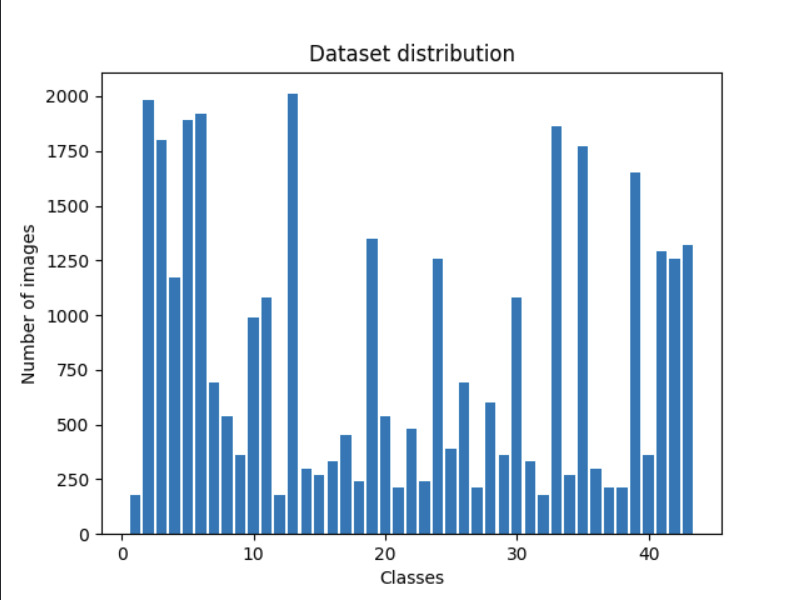
\includegraphics[width=\linewidth,trim=4 4 4 4,clip]{images/distribution.jpeg}
  \caption{Raspodijela dataseta po razredima.}
\end{figure}
\pagebreak
\section{Pretprocesiranje}
Pretprocesiranje ulaznog skupa podataka
\pagebreak
\section{Augmentacija skupa podataka}
Kako bi iskoristivost skupa podataka za treniranje bila maksimizirana korištena je augmentacija nad ulaznim skupom.
Augmentacija se provodi u sljedećem bloku programskog koda:
\\
\begin{lstlisting}[language=Python]
from keras.preprocessing.image import ImageDataGenerator


def augment():
    data_gen = ImageDataGenerator(width_shift_range=0.1,
                                  height_shift_range=0.1,
                                  zoom_range=0.2,
                                  shear_range=0.1,
                                  rotation_range=10)
    return data_gen
\end{lstlisting}

Gore prikazana funkcija koristi \code{ImageDataGenerator} funkciju iz
\\
\code{keras.preprocessing.image} modula. Uz navedene argumente ova metoda proširuje \emph{dataset} tako što svaku sliku
\begin{itemize}
	\item  Nasumično pomiče horizontalno uz maksimalni faktor od 10\% širine slike
	\item  Nasumično pomiče vertikalno uz maksimalni faktor od 10\% visine slike
	\item Uvečava sliku u rasponu od 0\% do 20\%
	\item  Posmiče slike uz maksimalni kut posmaka od 10\textdegree 
	\item  Rotira sliku uz maksimalni kut rotacije od 10\textdegree
\end{itemize}
\begin{figure}[h!]
  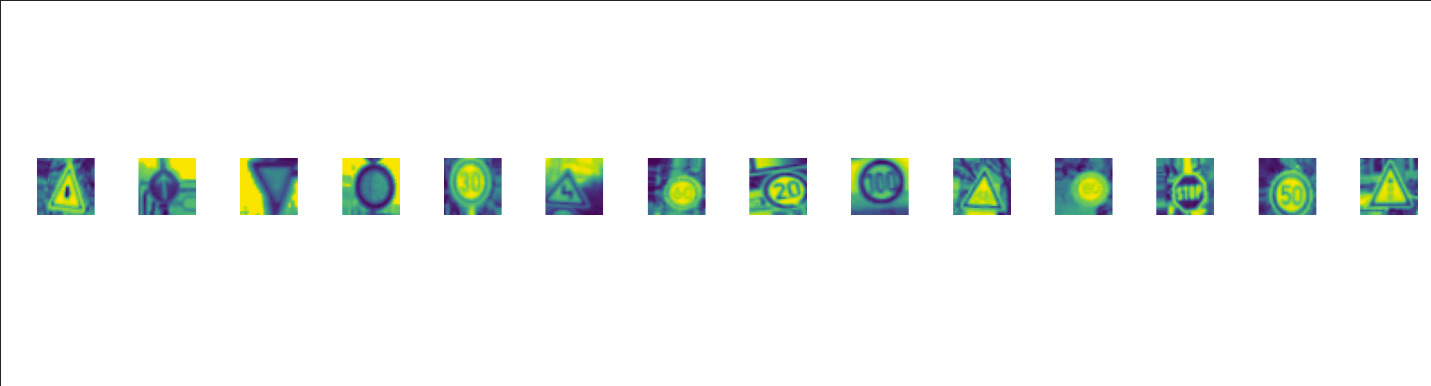
\includegraphics[width=\linewidth,trim=4 4 4 4,clip]{images/image-augmentation.jpeg}
  \caption{Prikaz augmentiranih slika.}
\end{figure}

\section{Treniranje modela}

\section{Testna aplikacija}


\chapter{Rezultati}

\chapter{Budući rad}

\chapter{Zaključak}
Zaključak.

\bibliography{literatura}
\bibliographystyle{fer}

\begin{sazetak}
Sažetak na hrvatskom jeziku.

\kljucnerijeci{Klasifikacija, računalni vid, strojno učenje, duboko učenje, duboke neuronske mreže, konvolucijske neuronske mreže, prometni znakovi, promet, DNN, CNN, CV, ML}

\end{sazetak}


\engtitle{Traffic sign classification}
\begin{abstract}
Abstract.

\keywords{Classification, Computer Vision, Machine Learning, Deep Learning, Deep Neural Networks, Convolutional Neural Networks, Traffic Signs, Traffic, DNN, CNN, CV, ML}

\end{abstract}

\end{document}
